\documentclass[journal,12pt,twocolumn]{IEEEtran}
%
\usepackage{setspace}
\usepackage{gensymb}
%\doublespacing
\singlespacing

%\usepackage{graphicx}
%\usepackage{amssymb}
%\usepackage{relsize}
\usepackage[cmex10]{amsmath}
\usepackage{siunitx}
%\usepackage{amsthm}
%\interdisplaylinepenalty=2500
%\savesymbol{iint}
%\usepackage{txfonts}
%\restoresymbol{TXF}{iint}
%\usepackage{wasysym}
\usepackage{amsthm}
\usepackage{iithtlc}
\usepackage{mathrsfs}
\usepackage{txfonts}
\usepackage{stfloats}
\usepackage{steinmetz}
\usepackage{supertabular}
%\usepackage{bm}
\usepackage{cite}
\usepackage{cases}
\usepackage{subfig}
%\usepackage{xtab}
\usepackage{longtable}
\usepackage{multirow}
%\usepackage{algorithm}
%\usepackage{algpseudocode}
\usepackage{enumitem}
\usepackage{mathtools}
\usepackage{tikz}
\usepackage{circuitikz}
\usepackage{verbatim}
\usepackage{tfrupee}
\usepackage[breaklinks=true]{hyperref}
%\usepackage{stmaryrd}
\usepackage{tkz-euclide} % loads  TikZ and tkz-base
%\usetkzobj{all}
\usetikzlibrary{calc,math}
\usetikzlibrary{fadings}
\usepackage{listings}
    \usepackage{color}                                            %%
    \usepackage{array}                                            %%
    \usepackage{longtable}                                        %%
    \usepackage{calc}                                             %%
    \usepackage{multirow}                                         %%
    \usepackage{hhline}                                           %%
    \usepackage{ifthen}                                           %%
  %optionally (for landscape tables embedded in another document): %%
    \usepackage{lscape}     
\usepackage{multicol}
\usepackage{chngcntr}
\usepackage{blkarray}
\usepackage{karnaugh-map}
\usepackage{fontspec}
\usepackage[intoc]{nomencl}
\makenomenclature

%\usetikzlibrary{arrows, shapes.gates.logic.US, calc}
\usetikzlibrary{arrows,shapes.gates.logic.US,shapes.gates.logic.IEC,calc}
\setmainfont{hindi/fonts/Sanskrit_2003.ttf}
%\setmainfont{Nakula.ttf}
%\setmainfont{Lohit-Devanagari.ttf}


%\usepackage{enumerate}

%\usepackage{wasysym}
%\newcounter{MYtempeqncnt}
\DeclareMathOperator*{\Res}{Res}
%\renewcommand{\baselinestretch}{2}
\renewcommand\thesection{\arabic{section}}
\renewcommand\thesubsection{\thesection.\arabic{subsection}}
\renewcommand\thesubsubsection{\thesubsection.\arabic{subsubsection}}

\renewcommand\thesectiondis{\arabic{section}}
\renewcommand\thesubsectiondis{\thesectiondis.\arabic{subsection}}
\renewcommand\thesubsubsectiondis{\thesubsectiondis.\arabic{subsubsection}}

% correct bad hyphenation here
\hyphenation{op-tical net-works semi-conduc-tor}
\def\inputGnumericTable{}                                 %%


\lstset{
%language=shell,
%language = Prolog,
frame=single, 
breaklines=true,
%showstringspaces=false,
columns=fullflexible
literate = {-}{-}1
}
%\lstset{
%language=tex,
%frame=single, 
%breaklines=true
%}

\begin{document}
%


\newtheorem{theorem}{Theorem}[section]
\newtheorem{problem}{Problem}
\newtheorem{proposition}{Proposition}[section]
\newtheorem{lemma}{Lemma}[section]
\newtheorem{corollary}[theorem]{Corollary}
\newtheorem{example}{Example}[section]
\newtheorem{definition}[problem]{Definition}
%\newtheorem{thm}{Theorem}[section] 
%\newtheorem{defn}[thm]{Definition}
%\newtheorem{algorithm}{Algorithm}[section]
%\newtheorem{cor}{Corollary}
\newcommand{\BEQA}{\begin{eqnarray}}
\newcommand{\EEQA}{\end{eqnarray}}
\newcommand{\define}{\stackrel{\triangle}{=}}

\bibliographystyle{IEEEtran}
%\bibliographystyle{ieeetr}


\providecommand{\mbf}{\mathbf}
\providecommand{\pr}[1]{\ensuremath{\Pr\left(#1\right)}}
\providecommand{\qfunc}[1]{\ensuremath{Q\left(#1\right)}}
\providecommand{\sbrak}[1]{\ensuremath{{}\left[#1\right]}}
\providecommand{\lsbrak}[1]{\ensuremath{{}\left[#1\right.}}
\providecommand{\rsbrak}[1]{\ensuremath{{}\left.#1\right]}}
\providecommand{\brak}[1]{\ensuremath{\left(#1\right)}}
\providecommand{\lbrak}[1]{\ensuremath{\left(#1\right.}}
\providecommand{\rbrak}[1]{\ensuremath{\left.#1\right)}}
\providecommand{\cbrak}[1]{\ensuremath{\left\{#1\right\}}}
\providecommand{\lcbrak}[1]{\ensuremath{\left\{#1\right.}}
\providecommand{\rcbrak}[1]{\ensuremath{\left.#1\right\}}}
\providecommand{\ceil}[1]{\left \lceil #1 \right \rceil }
\theoremstyle{remark}
\newtheorem{rem}{Remark}
\newcommand{\sgn}{\mathop{\mathrm{sgn}}}
\providecommand{\abs}[1]{\left\vert#1\right\vert}
\providecommand{\res}[1]{\Res\displaylimits_{#1}} 
\providecommand{\norm}[1]{\left\lVert#1\right\rVert}
%\providecommand{\norm}[1]{\lVert#1\rVert}
\providecommand{\mtx}[1]{\mathbf{#1}}
\providecommand{\mean}[1]{E\left[ #1 \right]}
\providecommand{\fourier}{\overset{\mathcal{F}}{ \rightleftharpoons}}
%\providecommand{\hilbert}{\overset{\mathcal{H}}{ \rightleftharpoons}}
\providecommand{\system}{\overset{\mathcal{H}}{ \longleftrightarrow}}
	%\newcommand{\solution}[2]{\textbf{Solution:}{#1}}
\newcommand{\solution}{\noindent \textbf{Solution: }}
\newcommand{\cosec}{\,\text{cosec}\,}
\providecommand{\dec}[2]{\ensuremath{\overset{#1}{\underset{#2}{\gtrless}}}}
\newcommand{\myvec}[1]{\ensuremath{\begin{pmatrix}#1\end{pmatrix}}}
\newcommand{\mydet}[1]{\ensuremath{\begin{vmatrix}#1\end{vmatrix}}}
%\numberwithin{equation}{section}
\numberwithin{equation}{subsection}
%\numberwithin{problem}{section}
%\numberwithin{definition}{section}
\makeatletter
\@addtoreset{figure}{problem}
\makeatother

\let\StandardTheFigure\thefigure
\let\vec\mathbf
%\renewcommand{\thefigure}{\theproblem.\arabic{figure}}
%\renewcommand{\thefigure}{\theproblem}
\renewcommand{\thefigure}{\thesection}
%\setlist[enumerate,1]{before=\renewcommand\theequation{\theenumi.\arabic{equation}}
%\counterwithin{equation}{enumi}


%\renewcommand{\theequation}{\arabic{subsection}.\arabic{equation}}

\def\putbox#1#2#3{\makebox[0in][l]{\makebox[#1][l]{}\raisebox{\baselineskip}[0in][0in]{\raisebox{#2}[0in][0in]{#3}}}}
     \def\rightbox#1{\makebox[0in][r]{#1}}
     \def\centbox#1{\makebox[0in]{#1}}
     \def\topbox#1{\raisebox{-\baselineskip}[0in][0in]{#1}}
     \def\midbox#1{\raisebox{-0.5\baselineskip}[0in][0in]{#1}}

\vspace{3cm}

\title{
%	\logo{
रेखीय बीजगणित
%	}
}
\author{ गाड़ेपल्लि वेंकट विश्वनाथ शर्मा $^{*}$% <-this % stops a space
	\thanks{*रचयिता भारतीय प्रौद्योगिकी संस्थान, हैदराबाद,५०२२८५ के विद्युत अभियान्त्रिकी विभाग में कार्यरत हैं, ईमेल:gadepall@ee.iith.ac.in। यह लेख मुक्त स्रोत विचारधारा के अनुरूप  है।}
	
}	
%\title{
%	\logo{Matrix Analysis through Octave}{\begin{center}\includegraphics[scale=.24]{tlc}\end{center}}{}{HAMDSP}
%}


% paper title
% can use linebreaks \\ within to get better formatting as desired
%\title{Matrix Analysis through Octave}
%
%
% author names and IEEE memberships
% note positions of commas and nonbreaking spaces ( ~ ) LaTeX will not break
% a structure at a ~ so this keeps an author's name from being broken across
% two lines.
% use \thanks{} to gain access to the first footnote area
% a separate \thanks must be used for each paragraph as LaTeX2e's \thanks
% was not built to handle multiple paragraphs
%

%\author{<-this % stops a space
%\thanks{}}
%}
% note the % following the last \IEEEmembership and also \thanks - 
% these prevent an unwanted space from occurring between the last author name
% and the end of the author line. i.e., if you had this:
% 
% \author{....lastname \thanks{...} \thanks{...} }
%                     ^------------^------------^----Do not want these spaces!
%
% a space would be appended to the last name and could cause every name on that
% line to be shifted left slightly. This is one of those "LaTeX things". For
% instance, "\textbf{A} \textbf{B}" will typeset as "A B" not "AB". To get
% "AB" then you have to do: "\textbf{A}\textbf{B}"
% \thanks is no different in this regard, so shield the last } of each \thanks
% that ends a line with a % and do not let a space in before the next \thanks.
% Spaces after \IEEEmembership other than the last one are OK (and needed) as
% you are supposed to have spaces between the names. For what it is worth,
% this is a minor point as most people would not even notice if the said evil
% space somehow managed to creep in.



% The paper headers
%\markboth{Journal of \LaTeX\ Class Files,~Vol.~6, No.~1, January~2007}%
%{Shell \MakeLowercase{\textit{et al.}}: Bare Demo of IEEEtran.cls for Journals}
% The only time the second header will appear is for the odd numbered pages
% after the title page when using the twoside option.
% 
% *** Note that you probably will NOT want to include the author's ***
% *** name in the headers of peer review papers.                   ***
% You can use \ifCLASSOPTIONpeerreview for conditional compilation here if
% you desire.




% If you want to put a publisher's ID mark on the page you can do it like
% this:
%\IEEEpubid{0000--0000/00\$00.00~\copyright~2007 IEEE}
% Remember, if you use this you must call \IEEEpubidadjcol in the second
% column for its text to clear the IEEEpubid mark.



% make the title area
\maketitle

\newpage

\tableofcontents


\bigskip

\renewcommand{\thefigure}{\theenumi}
\renewcommand{\thetable}{\theenumi}
\renewcommand{\abstractname}{सार}
\renewcommand{\nomname}{नामकरण}
\renewcommand{\solution}{हल: }
\renewcommand{\figurename}{आकृति.}
\renewcommand{\tablename}{सारणी.}
%\renewcommand{\theequation}{\theenumi}

%\begin{abstract}
%%\boldmath
%In this letter, an algorithm for evaluating the exact analytical bit error rate  (BER)  for the piecewise linear (PL) combiner for  multiple relays is presented. Previous results were available only for upto three relays. The algorithm is unique in the sense that  the actual mathematical expressions, that are prohibitively large, need not be explicitly obtained. The diversity gain due to multiple relays is shown through plots of the analytical BER, well supported by simulations. 
%
%\end{abstract}
% IEEEtran.cls defaults to using nonbold math in the Abstract.
% This preserves the distinction between vectors and scalars. However,
% if the journal you are submitting to favors bold math in the abstract,
% then you can use LaTeX's standard command \boldmath at the very start
% of the abstract to achieve this. Many IEEE journals frown on math
% in the abstract anyway.

% Note that keywords are not normally used for peerreview papers.
%\begin{IEEEkeywords}
%Cooperative diversity, decode and forward, piecewise linear
%\end{IEEEkeywords}



% For peer review papers, you can put extra information on the cover
% page as needed:
% \ifCLASSOPTIONpeerreview
% \begin{center} \bfseries EDICS Category: 3-BBND \end{center}
% \fi
%
% For peerreview papers, this IEEEtran command inserts a page break and
% creates the second title. It will be ignored for other modes.
%\IEEEpeerreviewmaketitle

\begin{abstract}
%इस आलेख में वामन को  दशक गणित्र के रूप में उपयोग करने का विधान प्रस्तुत है।
यह लेख लेटक के द्वारा देवनागरी में  वैज्ञानिक कृतियों  के लेखनविधि से आरम्भकर्ताओं को परिचित  कराने के प्रयास है ।


%ॐ श्री गणेशाय नमः॥
%\\
%\indent जय श्री राम।
%This manual provides a simple introduction to Digital Design.
\end{abstract}

%\section{Nomenclature}
\printnomenclature[1.7in]
%\addcontentsline{toc}{chapter}{Nomenclature}

%\nomenclature{Seven Segment Display}{ सप्तांश प्रदर्शी} 
%\nomenclature{Code}{ गूढ़} 
%\nomenclature{Decoder}{ गूढ़वाचक}
%\nomenclature{Incrementing}{ परवर्ती}
%\nomenclature{Decrementing}{ पूर्ववर्ती}
%\nomenclature{Karnaugh Map}{ कार्नो मानचित्र}
%\nomenclature{Implicant}{ विवक्षक}
%\nomenclature{LED}{ प्रकाश उत्सर्जक यंत्र}
%\nomenclature{Table}{ सारणी}
%\nomenclature{Figure}{ आकृति}
%\nomenclature{Variable}{ चर}
%\nomenclature{Input}{ आगत}
%\nomenclature{Output}{ निर्गत}
%\nomenclature{Boolean Algebra}{ बूलीय बीजगणित}
%\nomenclature{Verify}{ सत्यापित}
%\nomenclature{Combinational Logic}{ संयोजक तर्क}
%\nomenclature{Minimize}{ कनिष्ठीकरण}
%\nomenclature{Execute}{ निष्पादित, चालयन}
%\nomenclature{Expression}{ व्यंजक}
%\nomenclature{Equation}{ समीकरण}
%\nomenclature{Axiom}{ अभिगृह}
%\nomenclature{Reduced}{ समानयनिक}
%\nomenclature{C Program}{ C क्रमादेश}
%\nomenclature{Programming}{  क्रमादेशन}
%\nomenclature{Frequency}{ आवृत्ति}
%\nomenclature{Wordlength }{ मात्राभार}
%\nomenclature{Cable}{ रज्जु}
%\nomenclature{Button}{ गण्ड}
%\nomenclature{Left}{ वाम}
%\nomenclature{Right}{दक्षिण}
%\nomenclature{Blink}{श्मील}
%\nomenclature{IP Address}{अनिकेत}
%\nomenclature{Send}{प्रेषण}
%\nomenclature{File}{सञ्चिका}
%\nomenclature{Setup}{सप्रतिष्ठान}
%\nomenclature{Execute}{चालयन}
%\nomenclature{Interval}{अंतराल}

%\nomenclature{Binary}{ द्विआधारी}
%\nomenclature{Truth Table}{सत्य सारणी}
%\nomenclature{Derive}{व्युत्पन्न }
%\nomenclature{XOR}{अर्ध योग}
%\nomenclature{Complement}{पूरक}
%\nomenclature{Decade Counter}{दशक गणित्र}
%\nomenclature{Digital Logic}{अंकीय तर्क}
%\nomenclature{Function}{फलन}
%\nomenclature{Block Diagram}{खण्डारेख}
%\nomenclature{Circuit}{परिपथ}
%\nomenclature{Simplified Expression}{सरलीकृत व्यंजक}
%\nomenclature{Delay}{अतिकाल}
%\nomenclature{Minute}{निमिश}
%\nomenclature{Synchronous}{तुल्यकालिक}
%\nomenclature{Finite State Machine}{परिमित अवस्था यंत्र}
%\nomenclature{State Transition Table}{अवस्थान्तरण सारणी}
%\nomenclature{Flip flop}{द्विविध}
%\nomenclature{Design}{अभिकल्प}
%\nomenclature{Implementation}{कार्यान्वयन}
%\nomenclature{Period}{आवर्त}
%\nomenclature{Hardware}{यंत्रान्श}
%\nomenclature{Software}{तंंत्रान्श}
%\nomenclature{Computer}{संगणक}
%\nomenclature{Board}{परिपथफलक}
%\nomenclature{Port}{पत्तन}
%\nomenclature{Now}{इदान}
%\nomenclature{Weblink}{जालबन्धन}
%\nomenclature{Download}{अवाहरत}
%\nomenclature{Resistance}{प्रतिरोध}
%\nomenclature{Flash}{प्रस्फुरण}
%\nomenclature{Permutation}{क्रमचय}
%\nomenclature{Combination}{संचय}
\nomenclature{Point}{बिंदु}
\nomenclature{Vector}{सदिश}
\nomenclature{Matrix}{आव्यूह}
\nomenclature{Square}{वर्ग}
\nomenclature{Quadrilateral}{चतुर्भुज}
\nomenclature{Rectangle}{समचतुर्भुज}
\nomenclature{Parallelogram}{समांतर चतुर्भुज}
\nomenclature{Angle}{कोण}
\nomenclature{Scalar Product}{अदिश गुणनफल}







 

\section{बिंदु एवं सदिश}
%
\renewcommand{\theequation}{\theenumi}
\begin{enumerate}[label=\thesection.\arabic*.,ref=\thesection.\theenumi]
\numberwithin{equation}{enumi}
\numberwithin{figure}{enumi}
\numberwithin{table}{enumi}


\item निम्न बिंदु किस चतुर्भुज के शीर्ष हैं? कारण सहित अपने उत्तर की पुष्टि करें ।
\begin{align}
\vec{P} = \myvec{-1\\-2}, \vec{Q} =\myvec{1\\0},
\vec{R} =\myvec{-1\\2}, \vec{S} =\myvec{-3\\0}
\end{align}
\solution
आकृति 	\ref{fig:3.5.4_quadrilateral1} में
\begin{align}
\label{eq:constr_vectors_quad1_PSQR}
 \vec{P} - \vec{S} &= 
 \vec{Q} - \vec{R} = \myvec{2\\-2}
\\
\vec {R} - \vec {S} &=
 \vec {Q} - \vec {P} = \myvec{2\\2}
\label{eq:constr_vectors_quad1_RSQP}
\end{align}
%
$PQRS$ की सम्मुख भुजायें  समांतर हैं । अतः वह एक समांतर चतुर्भुज है । इसके अतिरिक्त
\begin{align}
\norm{ \vec{P} - \vec{S}} &= 
\norm{ \vec{Q} - \vec{R}} 
\\
=\norm{\vec {R} - \vec {S}} &=
\norm{ \vec {Q} - \vec {P}} = 2\sqrt{2}
\end{align}
%
$\because$ चतुर्भुज कीे समस्त भुजायें समान हैं, समांतर चतुर्भुज एक समचतुर्भुज है ।   $PS$ एवं
$RS$ से कृत कोण
\begin{align}
\cos \theta = \frac{\brak{\vec{S}-\vec{P}}^{\top}\brak{\vec{S}-\vec{R}}}{\norm{\vec{S}-\vec{P}}^{\top}\norm{\vec{S}-\vec{R}}}
\end{align}
%
$\because $
\begin{align}
\brak{\vec{S}-\vec{P}}^{\top}\brak{\vec{S}-\vec{R}} = \myvec{2 & -2}\myvec{2\\2} = 0
\end{align}
उपरोक्त समीकरण में $^{\top}$ अदिश गुणनफल का चिन्ह है.
\eqref{eq:constr_vectors_quad1_PSQR} का  \eqref{eq:constr_vectors_quad1_RSQP} में प्रतिस्थापन पर
\begin{align}
\cos \theta = 0 \implies PS \perp RS
\end{align}
%
अतः समचतुर्भुज मूलतः एक वर्ग है। 
\begin{figure}[!ht]
	\centering
	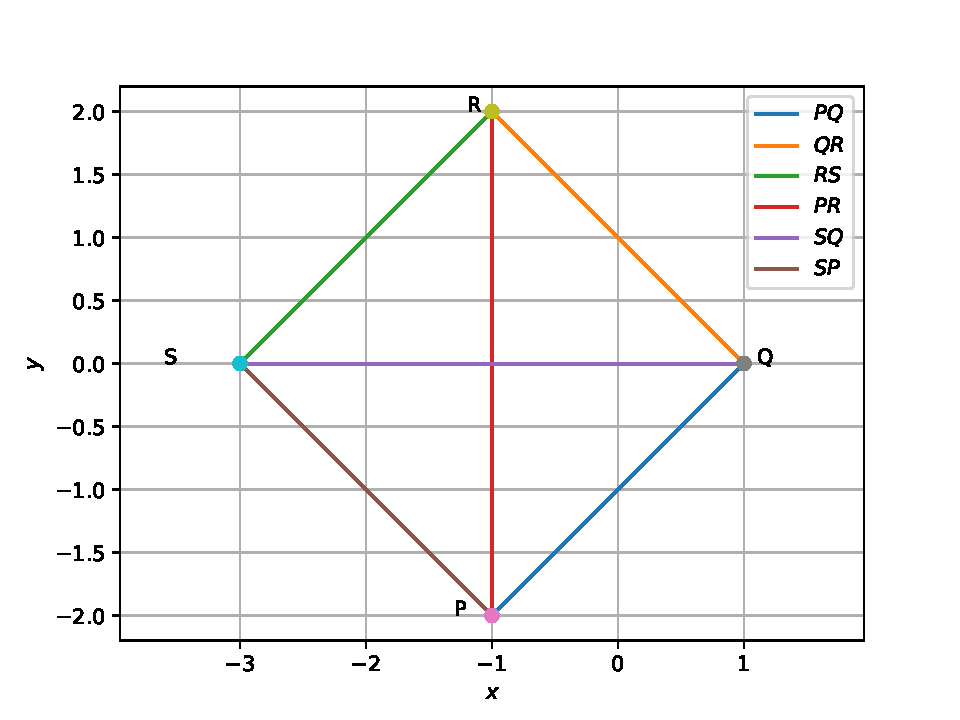
\includegraphics[width=\columnwidth]{figs/quad1.pdf}
	\caption{प्रदत्त बिंदुओं से एक वर्ग का निर्माण होता है।}
	\label{fig:3.5.4_quadrilateral1}
\end{figure}


\end{enumerate}

%\end{document}




%\section{तंत्रांश}
%इस आलेख के समस्त क्रमादेश निम्न जालबन्धन में उपलब्ध हैं।
%\begin{lstlisting}
%https://github.com/gadepall/vaman/tree/master/fpga/boolean/codes
%\end{lstlisting}
%%
%\section{सप्रतिष्ठान}
%\renewcommand{\theequation}{\theenumi}
%\renewcommand{\thefigure}{\theenumi}
%\begin{enumerate}[label=\thesection.\arabic*.,ref=\thesection.\theenumi]
%\numberwithin{equation}{enumi}
%\numberwithin{figure}{enumi}
%\numberwithin{table}{enumi}
%
%
%\item आकृति. \ref{fig:pin_sheet} में  वामन के समस्त कुशाव्यूह  प्रस्तुत हैं।  कुशाव्यूह J5 को  आकृति \ref{fig:sevenseg} में प्रदत्त सप्तांश प्रदर्शी के कुशों से सारणी \ref{table:vaman_dispdec} के द्वारा योजित करें। ध्यान  रहे कि COM एवं 3.3V के मध्य एक प्रतिरोधी अनिवार्य है। 
%\begin{table}[!ht]
%\centering
%\parbox{.45\columnwidth}{
%%\resizebox{0.5\columnwidth}{!}{
%\input{tables/vaman_sevenseg.tex}
%}
%\hfill
%\parbox{.45\columnwidth}{
%%\resizebox{0.5\columnwidth}{!}{
%\input{tables/vaman_dispdec.tex}
%}
%\caption{सप्तांश प्रदर्शी-वामन कुश योजना।}
%\label{table:vaman_dispdec}
%\end{table}
%
%\begin{figure}[!ht]
%\centering
%\resizebox{\columnwidth}{!}{
%\input{figs/sevenseg.tex}
%}
%\caption{सप्तांश प्रदर्शी}
%\label{fig:sevenseg}
%\end{figure}
%
%
%\begin{figure*}[!ht]
%\centering
%\includegraphics[width = \textwidth]{figs/pin_sheet.png}
%\caption{कुश आरेख}
%\label{fig:pin_sheet}
%\end{figure*}
%
%\item सारणी \ref{table:disp_dec} को वामन एवं सप्तांश प्रदर्शी से कार्यान्वित करें।
%\\
%\solution निम्न समीकरण में  सारणी \ref{table:disp_dec}  के निर्गत चर  $a,b,c,d,e,f,g$ की अभिव्यक्ति आगत चर $W,X,Y,Z$ के द्वारा की गयी है
%%
%\begin{align}
%\label{eq:disp_a}
%a &= WX^{\prime}Y^{\prime}Z^{\prime}+W^{\prime}X^{\prime}YZ^{\prime}
%\\
%\label{eq:disp_b}
%b &= WX^{\prime}YZ^{\prime}+W^{\prime}XYZ^{\prime}
%\\
%\label{eq:disp_c}
%c &= {Z}^{\prime}{Y}^{\prime}X{W}^{\prime}
%\\
%d &= WX^{\prime}Y^{\prime}Z^{\prime}+W^{\prime}X^{\prime}YZ^{\prime}+WXYZ^{\prime}+WX^{\prime}Y^{\prime}Z
%\label{eq:disp_d}
%\\
%e &= WX^{\prime}Y^{\prime}Z^{\prime}+WXY^{\prime}Z^{\prime}+W^{\prime}X^{\prime}YZ^{\prime}+WX^{\prime}YZ^{\prime}
%\nonumber \\
%&\quad +WXYZ^{\prime}+WX^{\prime}Y^{\prime}Z
%\label{eq:disp_e}
%\\
%f &= WX^{\prime}Y^{\prime}Z^{\prime}+W^{\prime}XY^{\prime}Z^{\prime}+WXY^{\prime}Z^{\prime}+WXYZ^{\prime}
%\label{eq:disp_f}
%\\
%g &= W^{\prime}X^{\prime}Y^{\prime}Z^{\prime}+WX^{\prime}Y^{\prime}Z^{\prime}+WXYZ^{\prime}
%\label{eq:disp_g}
%\end{align}
%\begin{table}
%\centering
%\input{./tables/disp_dec.tex}
%\caption{प्रदर्शी गूढ़वाचक की सत्य सारिणी ।}
%\label{table:disp_dec}
%\end{table}
%%
%निम्न क्रमादेश को इदान निष्पादित करें।
%\begin{lstlisting}
%codes/decoders/dispdec.v
%codes/decoders/pygmy.pcf
%\end{lstlisting}
%$W, X, Y, Z$ को GND से योजित करें।  तत्पश्चात चरों के भिन्न संचय के लिये प्रदर्शी में प्राप्त अंकों को सारणी \ref{table:disp_dec}  से सत्यापित करें।
%\item सारणी \ref{table:counter_decoder} में एक परवर्ती गूढ़वाचक के गुणधर्म का उल्लेख है।  बूलीय समीकरणों के द्वारा $A,B,C,D$ को $W,X,Y,Z$ के व्यञ्जकों में व्यक्त करें।  इसके पश्चात वामन के द्वारा परवर्ती गूढ़वाचक को कार्यान्वयित करें। 
%\label{prob:counter_decoder}
%\begin{table}
%\centering
%\input{./tables/counter_decoder.tex}
%\caption{परवर्ती गूढ़वाचक की सत्य सारिणी ।}
%\label{table:counter_decoder}
%\end{table}
%\\
%\solution निम्न समीकरणों में आवश्यक व्यञ्जक उपलब्ध हैं।
%\begin{align}
%\label{eq:inc_A}
%A &= W^{\prime}X^{\prime}Y^{\prime}Z^{\prime} + W^{\prime}XY^{\prime}Z^{\prime}
%+W^{\prime}X^{\prime}YZ^{\prime}
%\nonumber \\
% & \quad +W^{\prime}XYZ^{\prime}
%+W^{\prime}X^{\prime}Y^{\prime}Z
%\\
%\label{eq:inc_B}
%B &= WX^{\prime}Y^{\prime}Z^{\prime} + W^{\prime}XY^{\prime}Z^{\prime}
%\nonumber \\ 
%& \quad 
%+WX^{\prime}YZ^{\prime}
%+W^{\prime}XYZ^{\prime}
%\\
%\label{eq:inc_C}
%C &= WXY^{\prime}Z^{\prime} + W^{\prime}X^{\prime}YZ^{\prime}
%\nonumber \\ 
%& \quad 
%+WX^{\prime}YZ^{\prime}
%+W^{\prime}XYZ^{\prime}
%\\
%D &= WXYZ^{\prime} + W^{\prime}X^{\prime}Y^{\prime}Z
%\label{eq:inc_D}
%\end{align}
%निम्न क्रमादेश का चालयन करें। प्रदर्शी में परवर्ती अंक उत्पन्न होंगे।
%\begin{lstlisting}
%codes/decoders/incdec.v
%\end{lstlisting}
%\end{enumerate}
%%
%\section{दशक गणित्र}
%\renewcommand{\theequation}{\theenumi}
%\renewcommand{\thefigure}{\theenumi}
%\begin{enumerate}[label=\thesection.\arabic*.,ref=\thesection.\theenumi]
%\numberwithin{equation}{enumi}
%\numberwithin{figure}{enumi}
%\numberwithin{table}{enumi}
%
%\item आकृति. \ref{fig:vaman_decade_counter} के आधार पर क्रमादेश \ref{prob:counter_decoder}
%में संशोधन करें एवं वामन के द्वारा दशक गणित्र का निर्माण करें।
%\begin{figure}[!ht]
%\centering
%\resizebox{\columnwidth}{!}{
%\input{figs/vaman_decade_counter.tex}
%}
%\caption{दशक गणित्र का खंड आरेख.}
%\label{fig:vaman_decade_counter}
%\end{figure}
%\item पूर्ववतरी गूढ़वाचक की अभिकल्पना एवं कार्यान्वयन करें।
%
%\end{enumerate}
%

\end{document}



